\pagebreak
\subsection{Rysunki}
    \vspace{20px}
    \begin{figure}[ht]
        \centering
        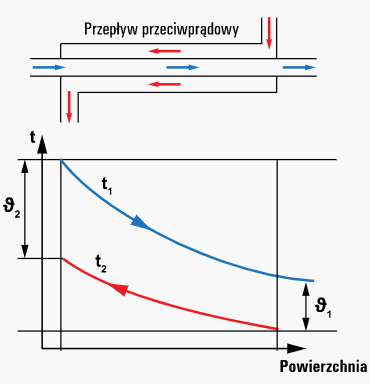
\includegraphics[width=\linewidth-250px]{Przeciwprąd.png}
            \caption{Uproszczony schemat wymiennika ''Rura w rurze'' w układzie przepływu przeciwprądowego oraz wykres przedstawiający temperaturę czynników dla takiego układu.\\
            \(t_{1we}=75\DEGc,t_{1wy}=55\DEGc,t_{2we}=30\DEGc,t_{2wy}=10\DEGc,\vartheta _1=45\DEGc,\vartheta _2=35\DEGc,\)}
        \centering
        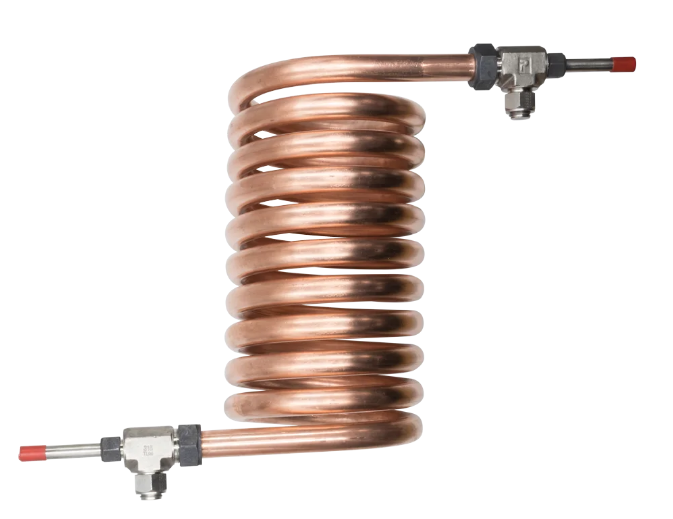
\includegraphics[width=\linewidth-250px]{Wymiennik.PNG}
            \caption{Poglądowy rysunek wymiennika typu ''Rura w rurze-rury zwijane''.}
    \end{figure}

